% !TEX encoding = UTF-8 Unicode
\documentclass[fontsize=11pt,paper=a4,titlepage,twoside,DIV=calc,draft=false]{scrbook}
% 11pt: Normale Textkörpergröße
% a4paper: Größe des Druckmediums
% titlepage: Titel auf einer separaten Seite ohne Seitenzahl
% twoside: Zweiseitiges Layout
% openright: Kapitel beginnen immer auf der rechten Seite
% headsepline: Trennt Textkörper von Headings durch Strich (entspr.: /footsepline)
% headinclude,footinclude: Kopf- und Fußzeile zählen zum Textkörper
% DIV=calc: Für die gewählten Optionen wird ein optimales Seitenverhältnis errechnet
% draft=true: Für Bilder wird die Box freigehalten, erheblicher Geschwindigkeitsvorteil.
% abstract: Setzt den Titel 'Zusammenfassung' vor den abstract

\usepackage{blindtext} 
\usepackage{upgreek}
%\usepackage{subfigure}

%  %  %  %  Bindungskorrektour  %  %  %  %
\KOMAoptions{BCOR=10mm}  


%  %  %  %  Abkürzungen  %  %  %  %
% Das Einführen dieser Befehler verhindert Umbrüche bei mehrgliedrigen Abkürzungen
\usepackage{xspace}
\newcommand{\zB}{\mbox{z.\,B.}\xspace}
% Abkürzung für zum Beispiel


%  %  %  %  Einheiten  %  %  %  %
\usepackage[thinspace,thinqspace,squaren,textstyle]{SIunits}
% Komfoatables Paket zum Einbinden von Einheiten


%  %  %  %  Kodierung, Schrift und Sprache  %  %  %  % 
\usepackage[utf8]{inputenc}
\usepackage{palatino}
\usepackage[ngerman]{babel}
% damit man Text aus dem PDF korrekt rauskopieren kann


%  %  %  %  Grafiken, Tabellen, Mathematikumgebungen  %  %  %  %
\usepackage{graphicx}
\usepackage{tabularx}
\usepackage{xcolor}
\definecolor{halfgray}{gray}{0.55} 
\usepackage{amsmath,amsfonts,amssymb}
\usepackage{flafter,afterpage}
\usepackage[section]{placeins}
\usepackage{setspace} \onehalfspacing
\usepackage[margin=8mm,font=small,labelfont=bf,format=plain]{caption}
\usepackage[margin=8mm,font=small,labelfont=bf,format=plain]{subcaption}

\numberwithin{equation}{chapter}
\numberwithin{figure}{chapter}
\numberwithin{table}{chapter}


%  %  %  %  Kopf- und Fußzeilen  %  %  %  %

\renewcommand\frontmatter{\pagenumbering{Roman}}
\usepackage{chngcntr} 
\counterwithout{footnote}{chapter}
  
  
% Zeilenabstand zwischen zwei Fußnoten:
\footnotesep9pt
% Einrücken der Fußnoten:
\deffootnote[1.5em]{1em}{1.5em}{\thefootnotemark\ \ }

\usepackage{fancyhdr}				% Paket für leicht konfigurierbare Kopf- und Fußzeilen
\fancypagestyle{plain}{				% Neue Gestaltung der Chapter- Page
\fancyhf{} 							% Clear all header and footer fields
\renewcommand{\headrulewidth}{0pt}	% Keine Trennlinie zwischen Kopf- / Fußzeile und Textkörper
\renewcommand{\footrulewidth}{0pt}}

\fancypagestyle{myfoot}{			% Neue Gestaltung der frontmatter pages
\fancyhf{}							% Clear all header and footer fields
\fancyhead[RO]{\thepage}			% Seitenzahl außen auf ungeraden Seiten
\fancyhead[LE]{\thepage}			% Seitenzahl außen auf geraden Seiten
\renewcommand{\headrulerwidth}{0pt}	% Keine Trennlinie zwischen Kopf- / Fußzeile und Textkörper
\renewcommand{\footrulerwidth}{0pt}}

\pagestyle{fancy}					% Pagestyle fancy aktiviert selbstkonfigurierten Style
\fancyhf{} 							% Alle Kopf- und Fußzeilenfelder werden zunächst bereinig
\renewcommand{\headrulewidth}{0pt}	% Keine Trennlienie zwischen Kopfzeile und Textkörper

\renewcommand{\chaptermark}[1]{\markboth{#1}{}}
%\renewcommand{\sectionmark}[1]{\markright{#1}{}}

\fancyhead[RO]{\leftmark ~~~~ \thepage}
\fancyhead[LE]{\thepage ~~~~ \nouppercase \rightmark}


%  %  %  %  Überschriften  %  %  %  %


%  %  %  %  Verzeichnisse  %  %  %  %

% % % Literaturverzeichnis % % %
%\usepackage{natbib}	

% % % Inhaltsverzeichnis % % %
% Die Chaptereinträge:
\usepackage{titletoc}

\titlecontents{chapter}
				[0pc]
				{\addvspace{0.5pc}%			
				%\filouter}
				}
				{\sffamily\LARGE\thecontentslabel\quad\sffamily\LARGE}{}
				{\titlerule*[0.75pc]{}\enskip\rmfamily\LARGE}%\contentspage}  % Wäre mit Seitenzahl 																					rechtsbündig
				[\addvspace{.5pc}]

% Die Sectioneinträge:
\titlecontents{section}
[3.78em]
{}
{\rmfamily\contentslabel{2.3em}\rmfamily}
{\hspace*{-2.3em}}
{\titlerule*[0.75pc]{.}\enskip\contentspage}
[\addvspace{.1em}]

% Die Subsectioneinträge:
\titlecontents{subsection}
[6.2em]
{}
{\rmfamily\contentslabel{2.3em}\rmfamily}
{\hspace*{-2.3em}}
{\titlerule*[0.75pc]{.}\enskip\contentspage}
[\addvspace{.1em}]

%\titlecontents{subsection}
%[6.8em]
%{}
%{\rmfamily\normalsize\contentslabel{3em}\rmfamily\large}
%{\hspace*{-2.3em}}
%{\titlerule*[0.75pc]{.}\enskip\contentspage}
\begin{document}

%  %  %  %  Titelseite  %  %  %  %
\begin{titlepage}
	\begin{tabularx}{\linewidth}{X}

		\\ \\ \hline

		\vspace{2em}

		\begin{singlespace}
			\begin{center}	\Large	\bfseries
				Software Engineering
			\end{center}
		\end{singlespace}

		\vspace{2em}

		\begin{singlespace}
			\begin{center}	\bfseries
 				Anforderungsanalyse zur Entwicklung
				eines SW-Systems zur Unterstützung
				der Einführung von Gleitarbeitszeit
			\end{center}
		\end{singlespace}

		\vspace{18em}

		\begin{center}
			vorgelegt von \\
			\vspace{2em}
 			Tom Graupner \\
			Markus Klemm \\
			Leonard Hecker
		\end{center}

		\vspace{2em}

		\\ \\ \hline

	\end{tabularx}
\end{titlepage}

%  %  %  %  Inhaltsverzeichnis  %  %  %  %

\tableofcontents

%  %  %  %  Hauptteil  %  %  %  %
\mainmatter

\chapter{Einführung}
Das Unternehmen \textsc{EKS}\footnote{Abkürzung für \textsc{Entwicklung von kundenspezifischer Software}} evaluiert aktuell die Umstellung ihres Arbeitszeitmodells zur Gleitzeit. Die Erfassung und Auswertung der Arbeitszeit soll dabei durch ein Software-System unterstützt werden. Die vorliegende Anforderungsanalyse beschäftigt sich zunächst mit den Rahmenbedingung und den Funktionen, die vom System übernommen werden sollen. Neben der Zusammenfassung aller funktionalen Anforderungen und der Struktur der Eigangs- und Ausgangsdaten, enthält diese Analyse verschiedene Anwendungsfalldiagramme\footnote{Als Abkürzung wird im folgenden \textsc{AWD} verwendet. Daran angelehnt ist die Abkürzung \textsc{AWF} für einen Anwendungsfall}, sowie ein Entity Relationship Model, welches die Speicherung der Daten veranschaulicht.

\chapter{Dokumentation der Anforderungen}
Anforderungen an ein Software-Produkt werden im Allgemeinen zunächst in funktionale und nicht-funktionale Anforderungen unterteilt. Erstere decken dabei die Fähigkeiten und die Beschaffenheiten ab, die der Benutzer der Software zur Problemlösung oder zur Erreichung seines Zieles benötigt. Nicht-funktionale Anforderungen unterteilen sich weiterhin in Rahmenbedingungen und Qualitätsanforderungen.

\section{Funktionale Anforderungen}
Die folgende Auflistung enthält die groben Funktionen, die vom Software-System erfüllt werden sollen. Bei einigen handelt es sich dabei um \textit{abstrakte Funktionen}, welche sich im weiteren Verlauf der Analyse feiner aufgliedern werden.

\begin{itemize}
	\item \textbf{Anwesenheit erfassen} \textit{\guillemotleft \ abstrakt \ \guillemotright}
	\item \textbf{Urlaub planen - Mitarbeiter} \textit{\guillemotleft \ abstrakt \ \guillemotright}
	\item \textbf{Urlaub verwalten - Abteilungsleiter} \textit{\guillemotleft \ abstrakt \ \guillemotright}
	\item \textbf{Krankheitsdaten erfassen}
	\item \textbf{Anwesenheit auswerten}
	\item \textbf{Zeitauswertung für Abteilungsleiter} \textit{\guillemotleft \ abstrakt \ \guillemotright}
\end{itemize}

\subsection{Tabellarischer überblick}
Die folgenden Tabellen fassen nun alle voneinander unabhängigen funktionalen Anforderungen an das Software-System zusammen. Im Rahmen der Anforderungsanalyse verwendet man für unabhängige funktionale Anforderungen ebenfalls den Begriff \textit{essentielle Funktionen}.

{
\vspace{1cm}
\hspace{-3,5cm}
\footnotesize
\begin{tabular}{|p{3cm}|p{4cm}|p{4cm}|p{4cm}|p{2cm}|}
	\hline
		\textbf{Funktion} &
		\textbf{Eingangsdaten} &
		\textbf{Ausgangsdaten} &
		\textbf{Bemerkungen} &
		\textbf{abstrakter AWD} \\
	\hline \hline
		\textit{Betreten} &
		MA-ID und Uhrzeit &
		Zutritt und Speicherung der Zeit, alternativ Zutrittsverweigerung &
		Bei einer ungültigen MA-ID kann der Zutritt verweigert werden &
		\textbf{Anwesenheit erfassen} \\
	\cline{1-4}
		\textit{Verlassen} &
		MA-ID und Uhrzeit &
		Verlassen und Speicherung der Zeit, alternative Fehlermeldung &
		&
		\\
	\cline{1-4}
		\textit{Wachdienst \mbox{informieren}} &
		Mitarbeiterliste &
		Detaillierte Information an den Wachdienst &
		Der Wachdienst wird stündlich darüber informiert, welche Mitarbeiter sich im Gebäude befinden &
		\\
	\hline
\end{tabular}
}

{
\vspace{0,5cm}
\hspace{-3,5cm}
\footnotesize
\begin{tabular}{|p{3cm}|p{4cm}|p{4cm}|p{4cm}|p{2cm}|}
	\hline
		\textit{Urlaub beantragen} &
		Urlaubswunsch &
		Urlaubsantrag &
		Urlaub wird unter Verwendung der eigenen MA-ID beim jeweiligen Abteilungsleiter beantragt &
		\textbf{Urlaub \newline planen, \newline Mitarbeiter } \\
	\cline{1-4}
		\textit{Urlaubsinformationen anzeigen} &
		Wunsch nach Urlaubsinformationen &
		Informationen zu Urlaubsterminen, Beantragungs\-status, verbrauchten und verbleibenden Urlaubstagen &
		&
		\\
	\cline{1-4}
		\textit{Urlaubsantrag \newline stornieren} &
		Storno-Wunsche &
		Storno-Bestätigung mit Aktualisierung der Urlaubsdaten &
		Mitarbeiter kann offene, abgelehnte und genehmigte (noch nicht angetretene) Urlaubsanträge stornieren &
		\\
	\cline{1-4}
		\textit{Urlaubsvorschlag annehmen} &
		Urlaubsvorschlag des Abteilungsleiter &
		 Aktualisierung der Urlaubsinformationen &
		Abteilungsleiter können Mitarbeiter ihrer Abt. Vorschläge unterbreiten &
		\\
	\cline{1-4}
		\textit{Urlaubsvorschlag \newline stornieren} &
		Urlaubsvorschlag des Abteilungsleiter und Storno-Wunsch &
		Stornierungsmitteilung und Aktualisierung der Urlaubsinformationen &
		Abteilungsleiter können Mitarbeitern ihrer Abt. Vorschläge unterbreiten &
		\\
	\hline
\end{tabular}
}

{
\hspace{-3,5cm}
\footnotesize
\begin{tabular}{|p{3cm}|p{4cm}|p{4cm}|p{4cm}|p{2cm}|}
	\hline
		\textbf{Funktion	} &
		\textbf{Eingangsdaten} &
		\textbf{Ausgangsdaten}&
		\textbf{Bemerkungen}	&
		\textbf{abstrakter AWD} \\
	\hline \hline
		\textit{Urlaubsantrag \newline genehmigen} &
		Urlaubsantrag eines MA &
		Aktualisierung der Urlaubsdaten und Bestätigung &
		Abteilungsleiter müssen Anträge ihrer Mitarbeiter genehmigen &
		\textbf{Urlaub \newline verwalten, \newline Abt.-Leiter } \\
	\cline{1-4}
		\textit{Urlaubsantrag \newline ablehnen} &
		Urlaubsantrag eines MA &
		Aktualisierung der Urlaubsdaten und Absage&
		Abteilungsleiter können Anträge ihrer Mitarbeiter ablehnen &
		\\
	\cline{1-4}
		\textit{Vorschlag \newline unterbreiten} &
		Urlaubsvorschlag des Abteilungsleiters &
		Urlaubsvorschlag an Mitarbeiter und Aktualisierung der Urlaubsinformationen &
		Abteilungsleiter können Mitarbeitern Urlaubsvorschläge unterbreiten &
		\\
	\cline{1-4}
		\textit{Urlaubsinformationen eines Mitarbeiters an\-zeigen} &
		Wunsch des Abteilungsleiters nach Urlaubsinformationen eines Mitarbeiters &
		Detaillierte Informationen zur Abteilung &
		Abteilungsleiter können sich zur Entscheidungs\-unterstützung die Urlaubs\-informationen eines Mitarbeiters anzeigen lassen &
		\\
	\hline
\end{tabular}
}

{
\vspace{0,5cm}
\hspace{-3,5cm}
\footnotesize
\begin{tabular}{|p{3cm}|p{4cm}|p{4cm}|p{4cm}|p{2cm}|}
	\hline
		\textit{Krankmeldung \newline erfassen} &
		Krankenschein eines Mitarbeiters &
		Aktualisierung der Urlaubsinformationen &
		Sachbearbeiter (HR) erfasst Krankmeldungen von Mitarbeitern und betroffene Urlaubsinformationen werden sofort aktualisiert &
		 \\
	\hline
\end{tabular}
}

{
\vspace{0,5cm}
\hspace{-3,5cm}
\footnotesize
\begin{tabular}{|p{3cm}|p{4cm}|p{4cm}|p{4cm}|p{2cm}|}
	\hline
		\textit{Anwesenheit \newline auswerten} &
		Anwesenheitsinformationen eines Mitarbeiters &
		Detaillierte Arbeitszeit\-aus\-wertung des Mitarbeiters &
		Die Auswertung wird wöchentlich automatisch erstellt und dem Mitarbeiter per Email zugesandt &
		 \\
	\hline
\end{tabular}
}

{
\hspace{-3,5cm}
\footnotesize
\begin{tabular}{|p{3cm}|p{4cm}|p{4cm}|p{4cm}|p{2cm}|}
	\hline
		\textbf{Funktion	} &
		\textbf{Eingangsdaten} &
		\textbf{Ausgangsdaten}&
		\textbf{Bemerkungen}	&
		\textbf{abstrakter AWD} \\
	\hline \hline
		\textit{Gesamtbilanz \newline anfordern} &
		Wunsch nach Gesamtbilanz &
		Gesamtbilanz enthält detaillierte Informationen zur Arbeits\-zeit\-auswertung der Abteilung &
		Die Kennzahlen sind absolut und prozentual angegeben und betreffen einen beliebigen, abgelaufenen Zeitraum &
		\textbf{Zeitaus\-wertung für Abt.-Leiter}\\
	\cline{1-4}
		\textit{Urlaubszeitbilanz \newline anfordern} &
		Wunsch nach Urlaubsbilanz &
		Urlaubszeitbilanz enteält beantragte Urlaubstage der Abteilung in einem vorausschauenden Zeitraum &
		Anträge werden absolut und prozentual bezogen auf die Gesamtarbeitszeit dargestellt &
		\\
	\cline{1-4}
		\textit{Anwesenheitsliste \newline anfordern}&
		Wunsch nach Anwesenheitsliste &
		Liste enthält alle momentan anwesenden Mitarbeiter der eigenen Abteilung &
		&
		\\
	\hline
\end{tabular}
}

\vspace{1cm}

\subsection{Struktur der Eingangs- und Ausgangedaten}
Jede essentielle Funktion besitzt definierte Eingangs- und Ausgangsdaten. Die folgende Auflistung stellt die Struktur der entsprechenden Daten aller zuvor genannten essentiellen Funktionen dar.

{
\vspace{1cm}
\hspace{-2cm}
\footnotesize
\begin{tabular}{|p{3cm}|p{6cm}|p{6cm}|}
	\hline
		\textbf{Funktion	} &
		\textbf{Struktur der Eingangsdaten} &
		\textbf{Struktur der Ausgangsdaten} \\
	\hline \hline
		\textit{Betreten} &
		+ MA-ID \newline + Uhrzeit &
		Bestätigung des Zutritts und \newline Datensatz :=\{MA-ID, Uhrzeit\}, \newline alternativ Fehlermeldung \\
	\hline
		\textit{Verlassen} &
		+ MA-ID \newline + Uhrzeit &
		Bestätigung des Verlassen und \newline Datensatz :=\{MA-ID, Uhrzeit\}, \newline alternativ Fehlermeldung \\
	\hline
		\textit{Wachdienst \newline informieren} &
		Stündlicher Trigger zum Auslösen der Benachrichtigung&
		Detaillierte Mitarbeiterliste mit den Spalten \{MA-ID, Nachname, Vorname, Büro\} \\
	\hline
\end{tabular}
}

\newpage
% \thispagestyle{empty}
{
\hspace{-2cm}
\footnotesize
\begin{tabular}{|p{3cm}|p{6cm}|p{6cm}|}
	\hline
		\textbf{Funktion	} &
		\textbf{Struktur der Eingangsdaten} &
		\textbf{Struktur der Ausgangsdaten} \\
	\hline \hline
	\textit{Urlaub beantragen} &
		Urlaubswunsch := \{MA-ID, Liste: zu beantragende Urlaubstage\}&
		Urlaubsantrag := \{MA-ID, Nachname, Vorname, Liste: zu beantragende Urlaubstage\}\\
	\hline
		\textit{Urlaubsinformationen anzeigen} &
		Wunsch nach Urlaubsinformationen &
		Urlaubsinformationen := \{verbrauchte Urlaubstage, verbleibende Urlaubstage, Liste: Urlaubstermine inkl. Status (offen, genehmigt, abgelehnt\}\\
	\hline
		\textit{Urlaubsantrag \newline stornieren} &
		Urlaubsantrag s.o. (Status: offen / genehmigt und noch nicht angetreten).&
		Bestätigung der Stornierung und aktualisierte Urlaubsinformationen := \{verbrauchte Urlaubstage, verbleibende Urlaubstage, Liste: Urlaubstermine inkl. Status (offen, genehmigt, abgelehnt\}\\
	\hline
		\textit{Urlaubsvorschlag \newline annehmen} &
		Urlaubsvorschlag := \{MA-ID, Liste: vorgeschlagener Urlaubstage \}&
		Bestätigung des Urlaubsvorschlages und aktualisierte Urlaubsinformationen := \{verbrauchte Urlaubstage, verbleibende Urlaubstage, Liste: Urlaubstermine inkl. Status (offen, genehmigt, abgelehnt\}\\
	\hline
		\textit{Urlaubsvorschlag \newline stornieren} &
		Urlaubsvorschlag s.o.&
		Bestätigung des Urlaubsvorschlages und aktualisierte Urlaubsinformationen := \{verbrauchte Urlaubstage, verbleibende Urlaubstage, Liste: Urlaubstermine inkl. Status (offen, genehmigt, abgelehnt\}\\
	\hline
	\hline
		\textit{Urlaubsantrag \newline genehmigen} &
		Urlaubsantrag s.o. &
		Bestätigung der Genehmigung und aktualisierte Urlaubsinformationen := \{verbrauchte Urlaubstage, verbleibende Urlaubstage, Liste: Urlaubstermine inkl. Status (offen, genehmigt, abgelehnt\}\\
	\hline
		\textit{Urlaubsantrag \newline ablehnen} &
		Urlaubsantrag s.o. &
		Bestätigung der Ablehnung und aktualisierte Urlaubsinformationen := \{verbrauchte Urlaubstage, verbleibende Urlaubstage, Liste: Urlaubstermine inkl. Status (offen, genehmigt, abgelehnt\}\\
	\hline
		\textit{Urlaubsvorschlag \newline unterbreiten} &
		Wunsch einen Vorschlag zu unterbreiten oder konkreter Urlaubsantrag s.o.&
		Urlaubsvorschlag := \{MA-ID, Nachname, Vorname, Liste: vorgeschlagener Urlaubstage\} und aktualisierte Urlaubsinformationen := \{verbrauchte Urlaubstage, verbleibende Urlaubstage, Liste: Urlaubstermine inkl. Status (offen, genehmigt, abgelehnt\}\\
	\hline
		\textit{Urlaubsinformationen eines Mitarbeiters an\-zeigen} &
		Wunsch nach Urlaubsinformationen &
		Urlaubsinformationen := \{verbrauchte Urlaubstage, verbleibende Urlaubstage, Liste: Urlaubstermine inkl. Status (offen, genehmigt, abgelehnt\}\\
	\hline
\end{tabular}
}

{
\hspace{-2cm}
\footnotesize
\begin{tabular}{|p{3cm}|p{6cm}|p{6cm}|}
	\hline
		\textbf{Funktion	} &
		\textbf{Struktur der Eingangsdaten} &
		\textbf{Struktur der Ausgangsdaten} \\
	\hline \hline
		\textit{Krankmeldung erfassen} &
		Krankenschein eines \newline Mitarbeiters := \{Nachname, Vorname, Geburtsdatum, Zeitraum der Bescheinigung\} &
		Entsprechende Aktualisierung der Mitarbeiterdatensätze für Urlaubstage, Soll- und Ist-Arbeitszeit \\
	\hline \hline
		\textit{Anwesenheit \newline auswerten} &
		Arbeitsstunden, Urlaubstage und Krankmeldungen des Mitarbeiters&
		Detaillierte Arbeitszeitauswertung :=\{Soll-Arbeitszeit, Ist-Arbeitszeit, Stand des Arbeitszeitkontos \} \\
	\hline \hline
		\textit{Gesamtbilanz \newline anfordern} &
		Wunsch nach Gesamtbilanz &
		Gesamtbilanz zu Abteilung :=\{Sollarbeitszeit, tatsächliche Arbeitsstunden, Urlaubstage, Krankheitstage, überstunden\}\\
	\hline
		\textit{Urlaubsbilanz \newline anfordern} &
		Wunsch nach Urlaubsbilanz&
		Urlaubsbilanz der Abteilung :=\{beantragte Urlaubstage (absolut und prozentual bezogen auf Gesamtarbeitszeit)\}\\
	\hline
		\textit{Anwesenheitsliste \newline anfordern} &
		Wunsch nach Anwesenheitsliste &
		Anwesenheitsliste der Abteilung :=\{MA-ID, Nachname, Vorname, Arbeitsplatz\} \\
	\hline
\end{tabular}
}


\newpage
\section{Qualitätsanforderungen}
Nachdem weder interne, noch externe Qualitätsanforderungen explizit in den vorliegenden Rahmenbedingungen genannt sind, lautet die Aufgabe hier globale Anforderungen zu formulieren und eigene Gedanken zu entwickeln. \newline

Ein allgemeiner Punkt herausragender Bedeutung ist beispielsweise \newline \mbox{\textit{Datensicherheit und Integrität}}. Aufgrund der Sensibilität der zu verarbeitenden Daten und der mit ihnen verbundenen Business-Prozesse (e.g. Buchhaltung) ist unbedingt dafür zu sorgen, dass jegliche Daten \textit{zugriffssicher,} \textit{redundant} und unter \textit{definierten Integritätsbestimmungen} gespeichert und verarbeitet werden. \newline

Für die spätere Erweiterung oder Wartung der Software ist es au{\ss}erdem von gro{\ss}er Bedeutung, alle Funktionen und Komponenten des Systems lückenlos zu dokumentieren. \newline

Geht man etwas ins Detail und betrachtet die essentiellen Funktionen, so gibt es Punkte an denen die Benutzerfreundlichkeit deutlich verbessert werden kann. Empfohlen wären unter anderem \textit{Interaktionen mit der Software zu bestätigen}. Gemeint ist damit, dem Benutzer Rückmeldung zu erfolgreich oder nicht erfolgreich abgeschlossenen Interaktionen zu geben. \newline

Weitere vorstellbare Qualitätsanforderungen werden nach Bedarf mit dem Auftraggeber abgesprochen.

\newpage
\section{Rahmenbedingungen}
Als abschlie{\ss}ender Punkt der schriftlichen Formulierung der Anforderungen werden die Rahmenbedingungen festgehalten. Hierbei unterscheidet man zwischen \textit{technologischen}, \textit{rechtlichen} und \textit{organisatorischen Rahmenbedingungen}. \newline

Zu den \textit{technischen Rahmenbedingungen} gehört dabei, dass das System Zugriff auf den betriebsinternen Jahreskalender benötigt. Dies ist notwendig, um Feiertage und Betriebsruhetage automatisch in die Bilanz der Arbeitszeit\-konten einbeziehen zu können. Weiterhin sollen Urlaubstage und Krankmeldungen unmittelbar in die Bilanz einflie{\ss}en. \newline

Wichtigster Teil der \textit{rechtlichen Rahmenbedingungen} ist zweifelsohne das Thema Datensicherheit. Die Vollständigkeit und Integrität der personenbezogenen Daten muss zu jedem Zeitpunkt gewährleistet sein. Dies ist notwendig um Rechtssicherheit zu schaffen, für den Arbeitgeber und den Arbeitnehmer. \newline

Die \textit{organisatorischen Rahmenbedingungen} beinhalten vor allem Details zu den Arbeitszeitmodellen im Unternehmen. So besitzt ein Standard-Arbeitstag 8 Stunden und eine Arbeitswoche dementsprechenden 40 Stunden. Das Arbeitszeitkonto eines jeden Mitarbeiters wird dabei vom Beginn des Arbeitsverhältnisses an kumulativ geführt.

\newpage

\chapter{Kontextdiagramm}
Nach der ausführlichen Formulierung der Anforderungen folgt nun die Modellierung des SW-Systems. In einer ersten Abstraktion zeigt Abbildung \ref{Kontext} das entsprechenden \textit{Kontextdiagramm}. Es zeigt des System und dessen Schnittstellen zur Umwelt, sowie die Beziehungen zwischen den Benutzern.

\begin{figure}[hbp]
	\centering
	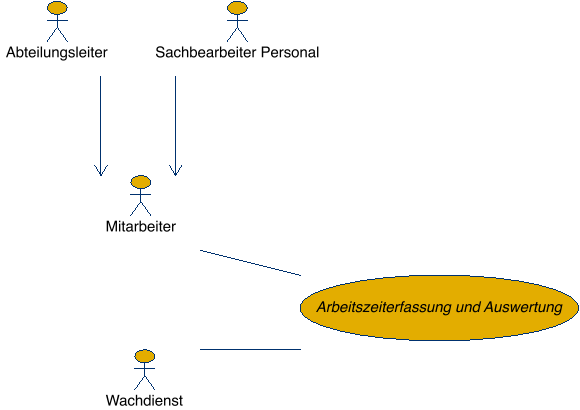
\includegraphics[width=0.9\linewidth]{UML/Export/Kontext.png}
	\caption{Kontextdiagramm zum SW-System \textit{Arbeitszeiterfassung und Auswertung}. Der Akteur Mitarbeiter generalisiert die Akteure Abteilungsleiter und Sachbearbeiter Personal}
	\label{Kontext}
\end{figure}

\chapter{Anwendungsfalldiagramme}
In einer weiteren Abstraktion werden die einzelnen Funktionen und ihre Kommunikationsbeziehungen zu den verschiedenen Akteuren dargestellt.

\section{AWD der groben Funktionalität}
Abbildung \ref{AWD} zeigt die oberste Abstraktionsebene der Anwendungsfalldiagramme. Die enthaltenen \textit{abstrakten Funktionen} Kapseln dabei mehrere verwandte Anwendungsfälle.

\vspace{1cm}
\begin{figure}[hbp]
	\centering
	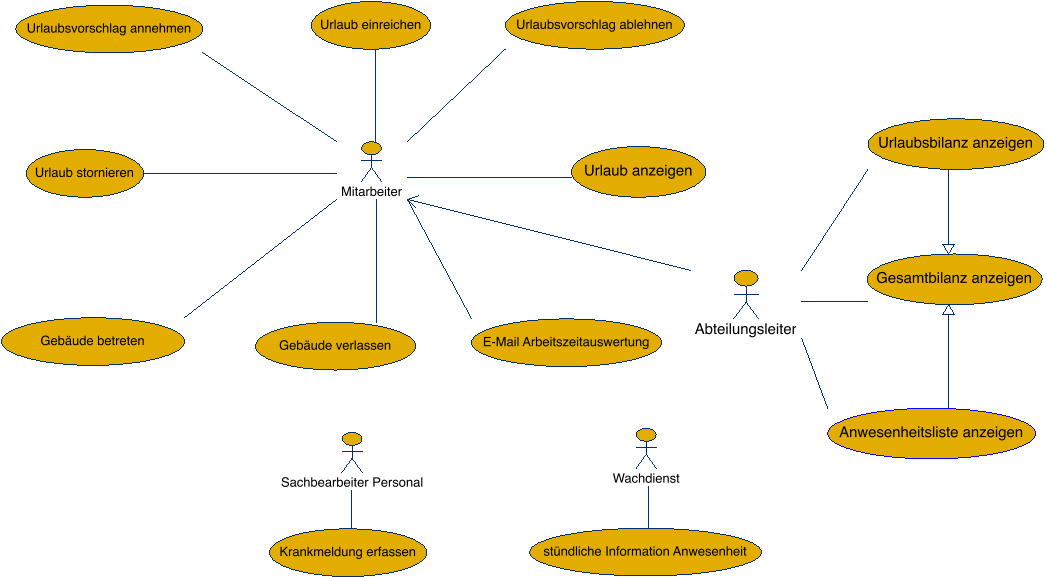
\includegraphics[width=\linewidth]{UML/Export/Grob.png}
	\caption{Anwendungsfalldiagramm zur groben übersicht.}
	\label{AWD}
\end{figure}

\newpage

\section{AWD der Funktionalität \textit{Urlaub planen}}
Beispielhaft wird nun die abstrakte Funktion \textit{Urlaub planen} näher betrachtet. Abbildung \ref{Urlaubplanen} zeigt das entsprechende AWD. Ein Mitarbeiter besitzt die Möglichkeiten Urlaub zu beantragen oder zu stornieren. Er kann weiterhin Urlaubsvorschläge seines Abteilungsleiters annehmen oder ebenfalls stornieren und seine persönlichen Urlaubsinformationen anzeigen.

\vspace{1cm}
\begin{figure}[hbp]
	\centering
	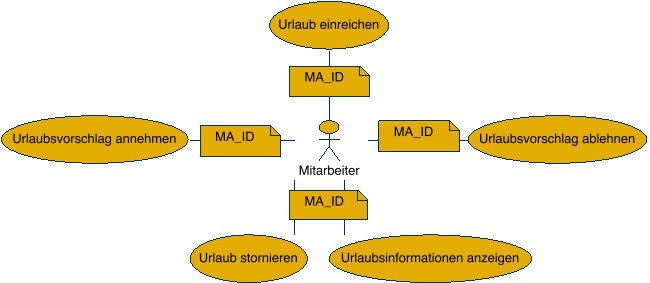
\includegraphics[width=\linewidth]{UML/Export/Urlaub_planen.png}
	\caption{Anwendungsfalldiagramm zur abstrakten Funktion \textit{Urlaub planen - Mitarbeiter}}
	\label{Urlaubplanen}
\end{figure}

\newpage

\section{Detaillierte Beschreibung der essentiellen Funktionalität \textit{Urlaub beantragen}}
Die essentielle Funktion \textit{Urlaub beantragen} gehört zu den kleinsten von anderen unabhängigen Anwendungsfällen. Beschreiben kann man sie wie folgt: \newline

Der Mitarbeiter verfasst seinen Urlaubsantrag, basierend auf seinen aktuellen Urlaubsinformationen. Der Antrag enthält die Daten MA-ID, Nachname, Vorname und eine Liste der zu beantragenden Urlaubstage. \newline

Nach \textsc{Chris Rupp} beschreibt man den Anwendungsfall alternativ unter Zuhilfenahme von Schatzschablonen folgenderma{\ss}en: \newline

SW-System \textit{Arbeitszeit erfassen und auswerten} muss dem Mitarbeiter die Möglichkeit bieten Urlaub einzureichen. \newline

Eine weitere Detaillierte Form der Modellierung bietet das Aktivitätsdiagramm. Es stellt die einzelnen Aktionen dar, die in einer Funktionalität gekapselt sind. Im Fall der essentiellen Funktionalität \textit{Urlaub beantragen} ist das Aktivitätsdiagramm trivial, dargestellt in Abbildung \ref{Aktivitaet}

\vspace{1cm}
\begin{figure}[hbp]
	\centering
	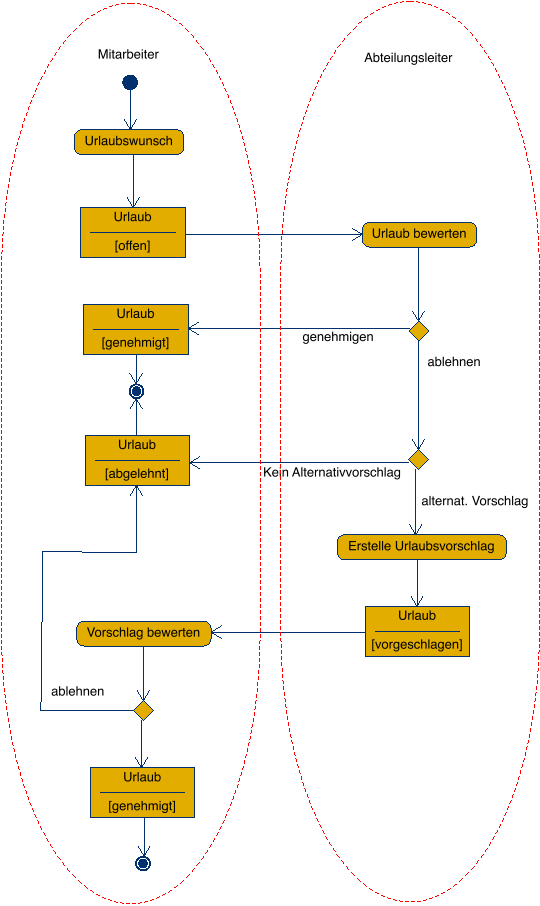
\includegraphics[width=\linewidth]{UML/Export/Urlaub_einreichen.png}
	\caption{Aktivitätsdiagramm der essentiellen Funktion \textit{Urlaub beantragen}.}
	\label{Aktivitaet}
\end{figure}

\chapter{Zustandsdiagramm eines Urlaubsantrages}
Der Anwendungsfall \textit{Urlaub planen} eines Mitarbeiters soll nun erneut detaillierter betrachtet werden. Dazu greifen wir das Objekt \textit{Urlaubsantrag} heraus und beschreiben es in einem Zustandsdiagramm genauer. Dieses Diagramm enthält die verschiedenen Zustände einer Betrachtungseinheit und beschreibt gleichzeitig die übergänge zwischen den Zuständen.

\vspace{1cm}
\begin{figure}[hbp]
	\centering
	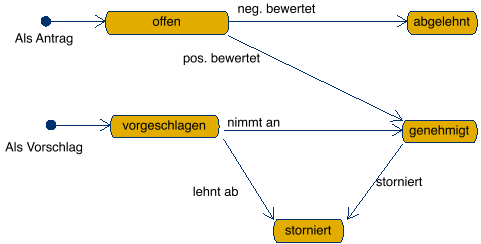
\includegraphics[width=0.9\linewidth]{UML/Export/Urlaubsantrag.png}
	\caption{Zustandsdiagramm des Objekts \textit{Urlaubsantrag}.}
	\label{Uantrag}
\end{figure}

\newpage

\chapter{Entity Relationship Model}

\begin{figure}[hbp]
	\centering
	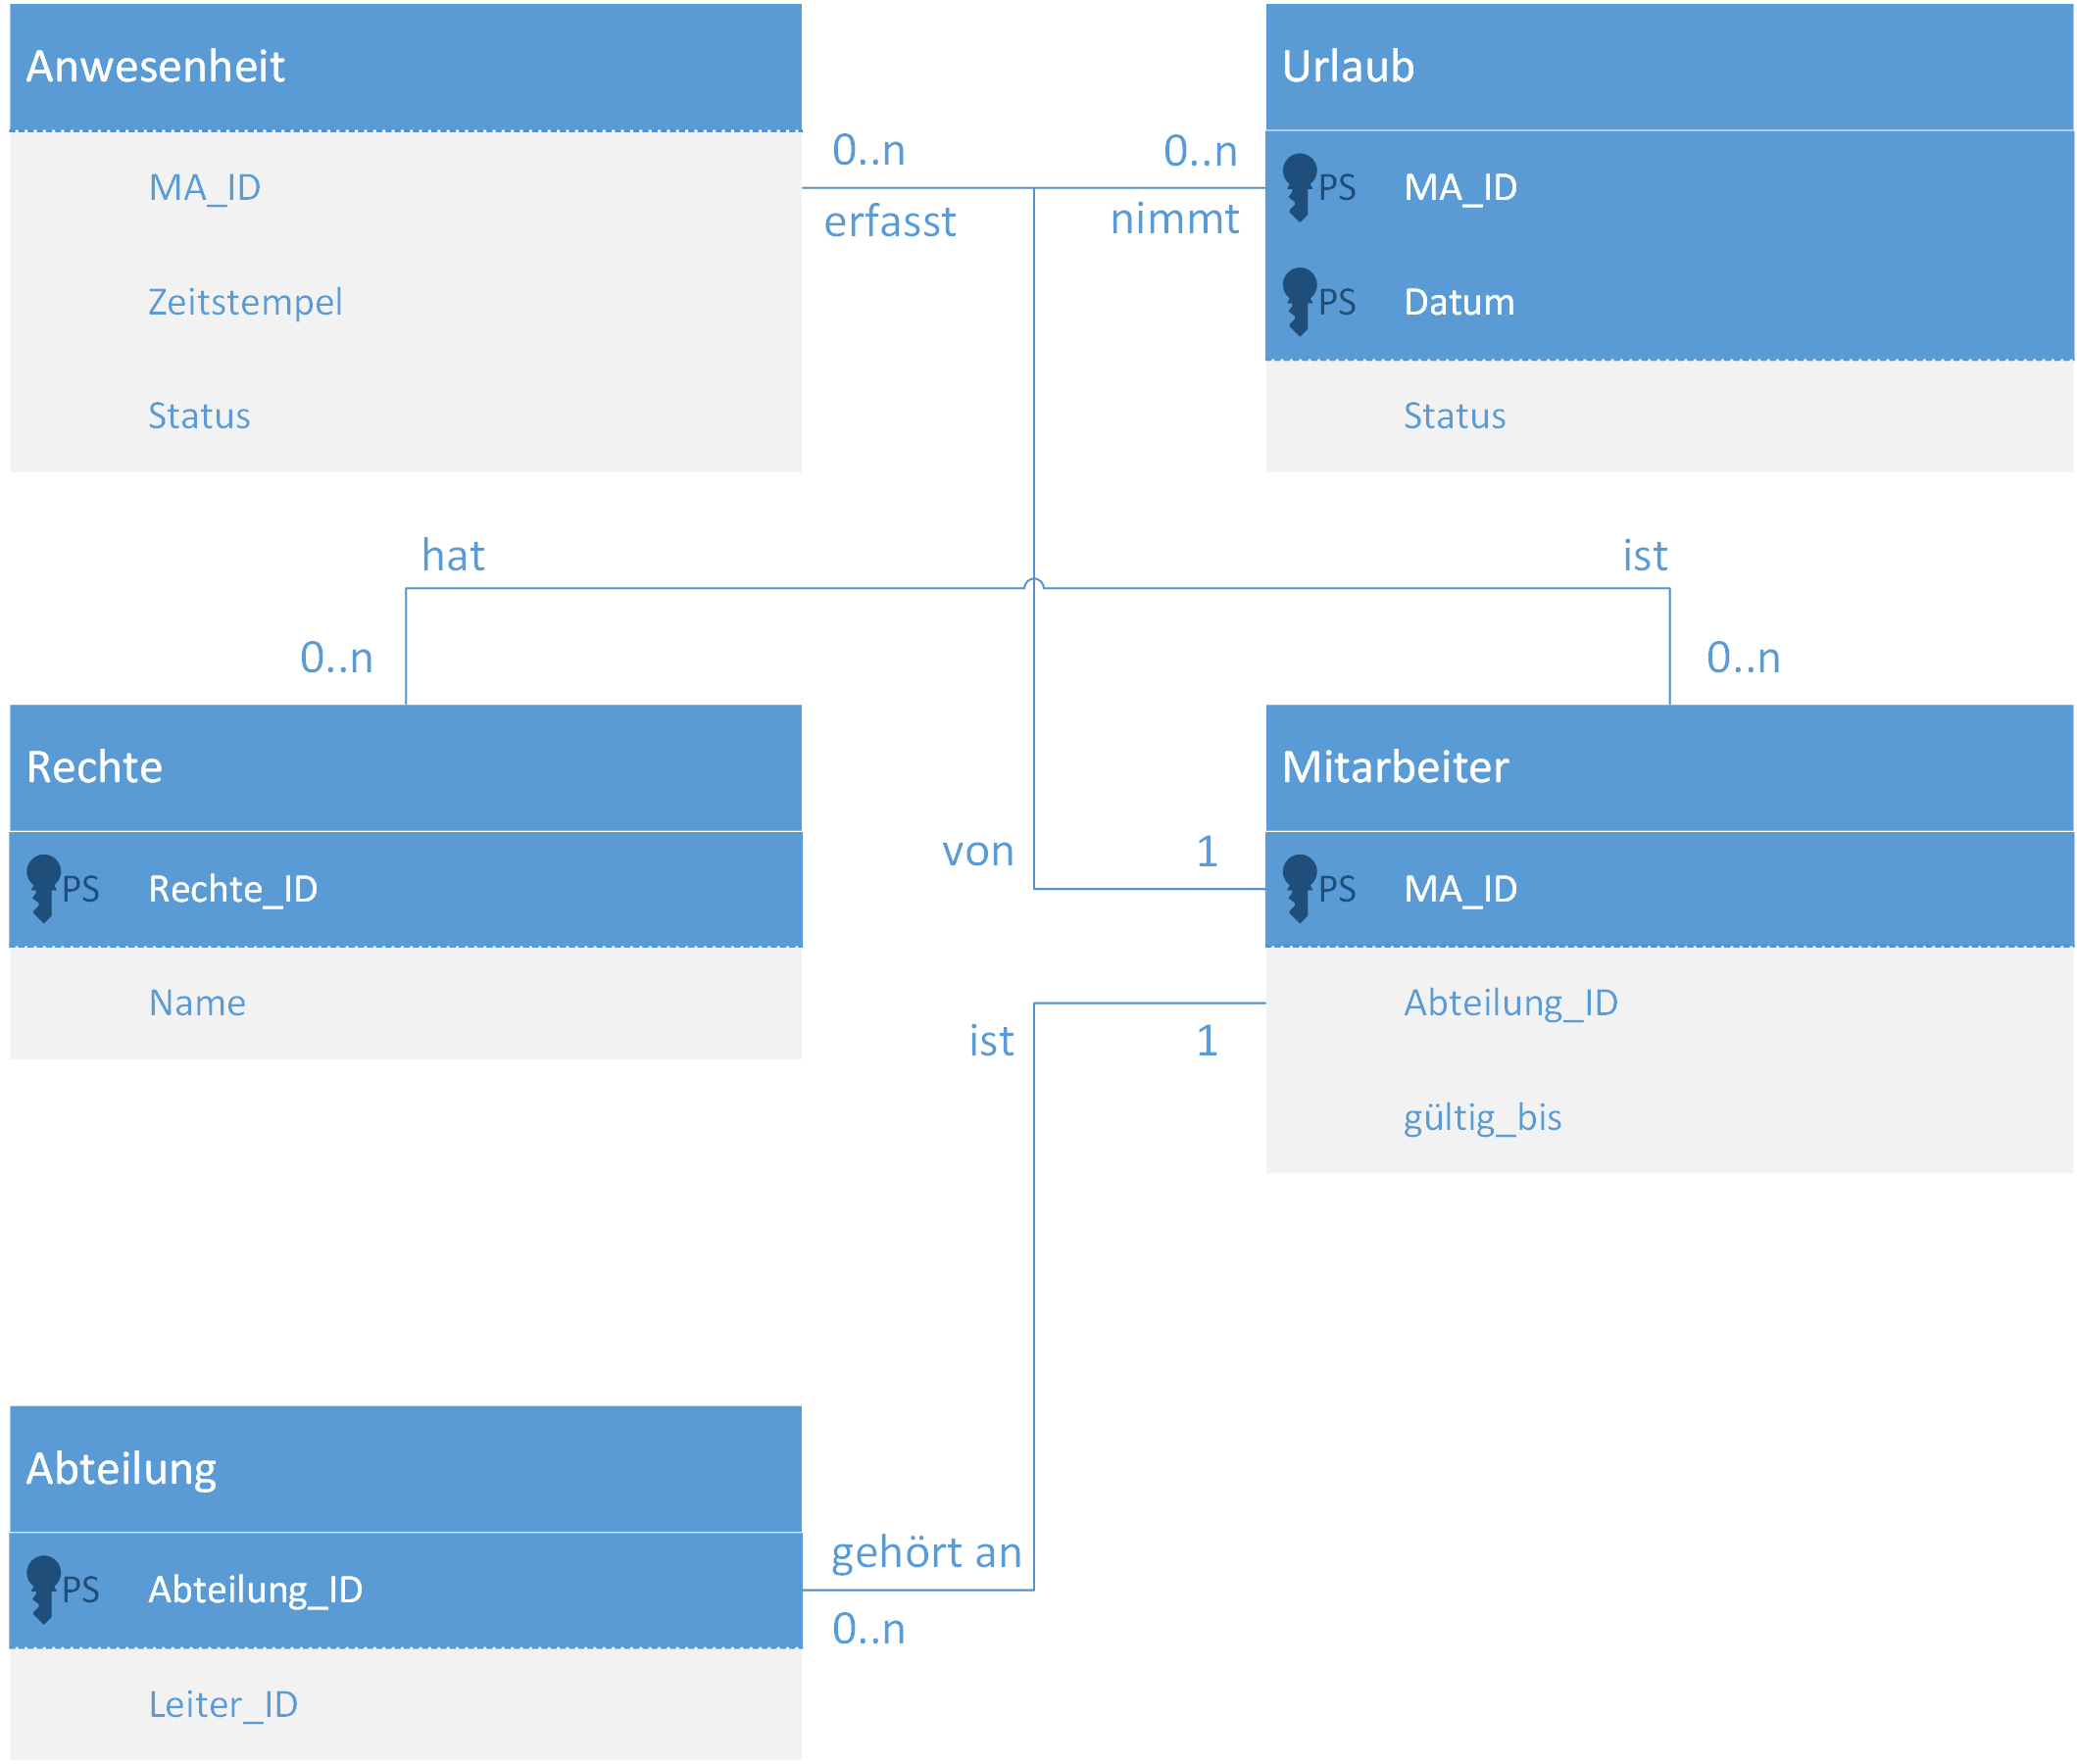
\includegraphics[width=1\linewidth]{UML/Export/erm.png}
	\caption{Entity Relationship Model aller essentiellen Funktionen}
	\label{ERM}
\end{figure}

\section{Detaillierte Beschreibung des Entity Relationship Model}
Die Tabelle Mitarbeiter enthält alle \textit{Mitarbeiter}, indiziert unter dem Primärschlüssel \textit{MA_ID}. Außerdem gibt es ein Attribut \textit{gültig_bis} um die Gültigkeit der Ausweise zu speichern. Die Tabelle könnte weitere Informationen enthalten, wie z.B. \enquote{Nachname}, \enquote{Vorname}, oder \enquote{Geburtsdatum}. \newline
Jeder Mitarbeiter ist einer beliebigen Anzahl an Abteilungen zugehörig, weshalb eine Tabelle \textit{Abteilung} existiert. Die Abteilungen der Firma sind unter dem Primärschlüssel \textit{Abteilung_ID} indiziert. Jede Abteilung besitzt einen Abteilungsleiter, der durch den Fremdschlüssel \textit{Leiter_ID}, welcher sich auf eine \textit{MA_ID} bezieht, beschrieben wird. \newline
Des Weiteren hat jeder Mitarbeiter eine beliebige Anzahl an Rechten, weshalb eine Tabelle \textit{Rechte} existiert. In dieser sind diese unter dem Primärschlüssel \textit{Rechte_ID} indiziert. Jedem Eintrag wird ein \textit{Name} zugeordnet, um in der Software auf den jeweiligen Eintrag über den Namen zuzugreifen. Dabei würde die Software z.B. die Verknüpfung von Rechte_ID auf Name umkehren und lokal zwischenspeichern, weshalb Rechte_ID als Primärschlüssel dennoch sinnvoll ist. \newline
Die Anwesenheitserfassung wird durch die Tabelle \textit{Erfassung} ermöglicht. Unter der \textit{MA_ID} und einem \textit{Zeitstempel} wird der \textit{Status} geloggt. \textit{MA_ID} bezieht sich hierbei als Fremdschlüssel auf einen Mitarbeiter und \textit{Status} enthält die Art des Eintrages, sprich \enquote{betreten} oder \enquote{verlassen}. Diese Tabelle enthält keinen Primärschlüssel, da MA_ID zusammen mit Zeitstempel und notfalls mit Status zwar praktisch einen Primärschlüssel bilden würden, jedoch nicht theoretisch. Da ein Primärschlüssel außerdem keinen Nutzen in dieser Tabelle hätte und um auch die theoretische Korrektheit zu gewähren, existiert deshalb keiner. Stattdessen sollte sich ein regulärer Index auf MA_ID und auf Zeitstempel für die Auswertung als nützlich erweisen. \newline
Zuletzt existiert die Tabelle \textit{Urlaub} um Urlaubsanträge zu erfassen. Diese werden hierbei unter dem zusammengesetzten Primärschlüssel aus \textit{MA_ID}, einem Fremdschlüssel, welcher sich auf einen Mitarbeiter bezieht, und \textit{Datum} des Urlaubstages. Möchte der Mitarbeiter mehrere Tage Urlaub nehmen so müssen mehrere Einträge in der Tabelle erstellt werden. Die Alternative ist es ein \enquote{Startdatum} und ein \enquote{Enddatum} des Urlaubs zu speichern. Das hier vorgeschlagene Konzept ist jedoch der Alternative überlegen, da es zwar mehr Einträge benötigt, dies jedoch die Implementierung stark vereinfacht und etwaige Fehler verhindert. Außerdem existiert ein Attribut \textit{Status} welcher den Status des Antrages enthält, sprich: \enquote{offen}, \enquote{abgelehnt}, oder \enquote{genehmigt}.

\newpage

\chapter{Glossar}
Der abschlie{\ss}ende Glossar soll es Personen aus verschiedenen Fachgebieten möglich machen, die vorliegende Anforderungsanalyse zu verstehen und mit ihr arbeiten zu können. Dazu werden wichtige Fachbegriffe aus dem Kontext des Software Engineering und der Anforderungsanalyse beschrieben.

\paragraph{Anwendungsfall}
Eine abstrakte Darstellung einer vom Software-System angebotenen Funktionalität (Aktivität). Er kapselt eine Menge von Aktionen, die sequentiell, bediengungsabhängig oder zyklisch abgearbeitet werden. Ein Anwendungsfall wird in Folge von Dateneingaben oder zeitlichen Ereignissen ausgelöst und führt in der Regel zu einem von au{\ss}en sichtbarem Ergebnis.

\paragraph{Anwendungsfalldiagramm}
Das Anwendungsfalldiagramm, kurz AWD, stellt die funktionalen Anforderungen (Aktivitäten) aus Sicht des Anwenders dar. Diese Aktivitäten werden zu den Beteiligten aus dem Kontext (Akteuren) in Beziehung gesetzt.

\paragraph{Akteur}
Ein Akteur ist die abstrakte Darstellung einer externen Instanz, die mit dem System kommuniziert.


\begin{itemize}
	\item abstrakte Funktion
	\item essentielle Funktion
	\item Entity Relationship Model
	\item Unified Modeling Language
	\item Mitarbeiter-ID
	\item t.b.c
\end{itemize}


\end{document}
